\begin{figure}[h!]
  \centering
  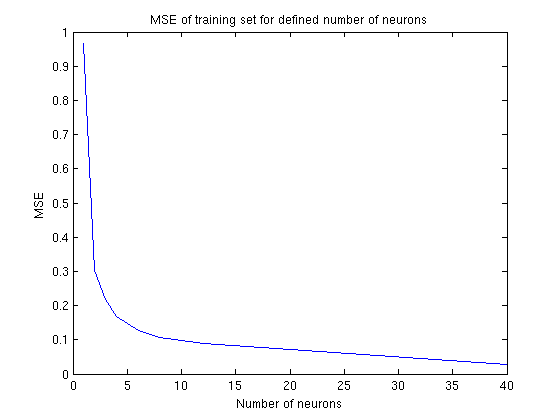
\includegraphics[width=0.75\textwidth]{./figures/3/3_mse_train.png}
  \caption{MSE für unterschiedliche Anzahl an Neuronen des Trainingssets}
  \label{fig:3_mse_train}
\end{figure}

\begin{figure}[h!]
  \centering
  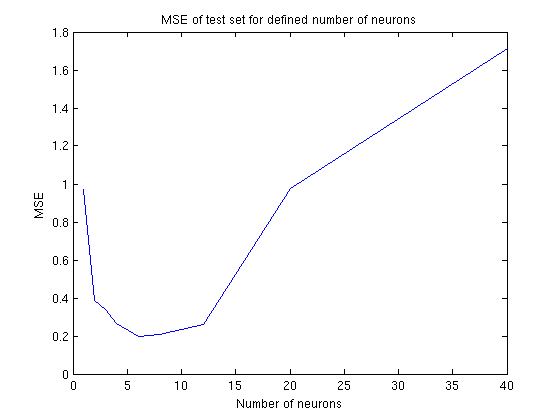
\includegraphics[width=0.75\textwidth]{./figures/3/3_mse_test.png}
  \caption{MSE für unterschiedliche Anzahl an Neuronen des Testsets}
  \label{fig:3_mse_test}
\end{figure}

Abbildungen \ref{fig:3_mse_train} und \ref{fig:3_mse_test} zeigen den Mean Squared Error (MSE) für unterschiedliche Neuronenanzahl bei den Trainings- bzw. Testdatensätzen. Man erkennt, dass der MSE bei den Trainingsdaten immer kleiner wird, je mehr Neuronen verwendet werden, da sich die entstehende Funktion des Neuronalen Netzwerks immer mehr den Trainingsdaten annähert. Betrachtet man allerdings den MSE der Testdaten, erkennt man, dass ab einer bestimmten Neuronenanzahl der Fehler wieder steigt. Dieser Effekt wird als \emph{Overfitting} bezeichnet, da das Neuronale Netzwerk versucht, die Trainingsdaten perfekt nachzubilden. Dadurch stimmt die gelernte Funktion nicht mehr mit der Zielfunktion überein.

Der beste Wert für $n$ wäre in diesem Fall 6, da hier der Fehler bei den Testdaten am geringsten ist. Für größere $n$ tritt Overfitting auf.

\begin{figure}[h!]
  \centering
  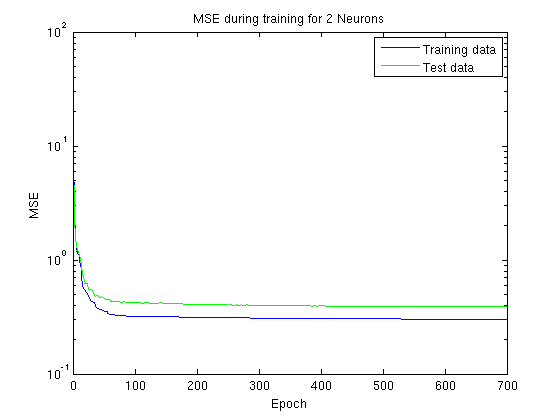
\includegraphics[width=0.7\textwidth]{./figures/3/3_mse_2.png}
  \caption{MSE des Trainings- und Testsets für 2 Neuronen}
  \label{fig:3_mse_2}
\end{figure}

\begin{figure}[h!]
  \centering
  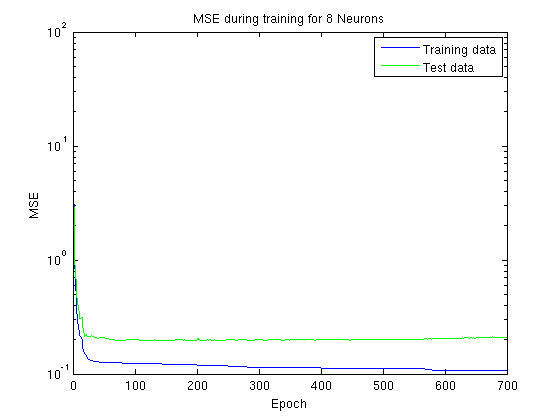
\includegraphics[width=0.7\textwidth]{./figures/3/3_mse_8.png}
  \caption{MSE des Trainings- und Testsets für 8 Neuronen}
  \label{fig:3_mse_8}
\end{figure}

\begin{figure}[h!]
  \centering
  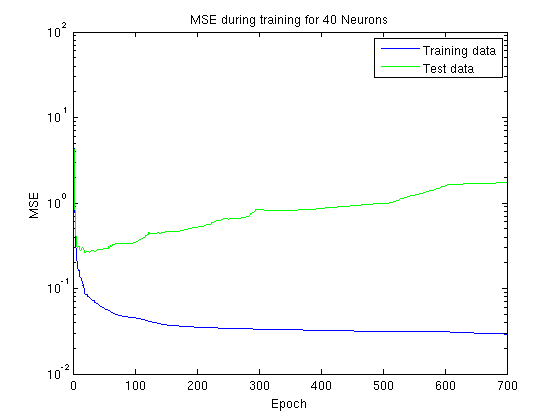
\includegraphics[width=0.7\textwidth]{./figures/3/3_mse_40.png}
  \caption{MSE des Trainings- und Testsets für 40 Neuronen}
  \label{fig:3_mse_40}
\end{figure}

Abbildungen \ref{fig:3_mse_2}, \ref{fig:3_mse_8} und \ref{fig:3_mse_40} zeigen den MSE auf den Trainings- und Testdaten für 2, 8, bzw. 40 Neuronen. Man erkennt, dass es bei niedriger Anzahl an Neuronen (hier: 2, Abb.~\ref{fig:3_mse_2}) keinen Overfitting-Effekt gibt, der verbleibende Fehler auf den Trainings- und Testdaten jedoch relativ hoch bleibt. Bei einer mittleren Anzahl an Neuronen (hier: 8, Abb.~\ref{fig:3_mse_8}) wird der Fehler auf den Trainings- und Testdaten kleiner, jedoch macht sich Overfitting bereits minimal bemerkbar. Bei einer hohen Anzahl an Neuronen (hier: 40, Abb.~\ref{fig:3_mse_40}) wird der Fehler auf den Trainingsdaten zwar sehr klein, durch Overfitting steigt der Fehler auf den Testdaten jedoch wieder stark an.

Der Fehler auf den Trainingsdaten nimmt mit zunehmender Anzahl Neuronen immer weiter ab, da die Funktion der Trainingsdaten immer genauer nachgebildet wird. Der Fehler auf den Testdaten steigt jedoch ab einer gewissen Anzahl Neuronen wieder, da der \emph{Overfitting}-Effekt auftritt.

\begin{figure}[h!]
  \centering
  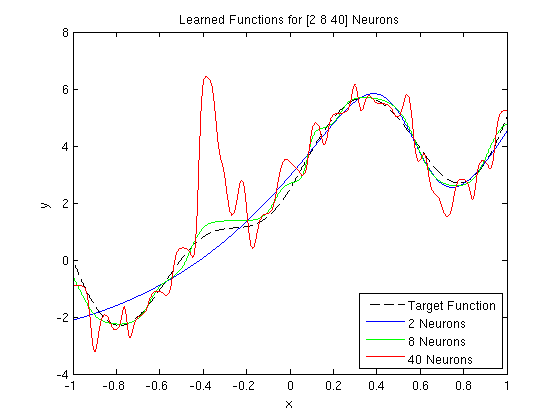
\includegraphics[width=0.75\textwidth]{./figures/3/3_learned.png}
  \caption{gelernte Funktion bei 2, 8 bzw. 40 Neuronen}
  \label{fig:3_learned}
\end{figure}

Abbildung~\ref{fig:3_learned} zeigt die gelernten Funktionen für 2, 8 bzw. 40 Neuronen. Wie man in den vorherigen Plots erkennt, ist die Annäherung an die Zielfunktion mit 2 Neuronen noch relativ schlecht, da der MSE noch sehr groß ist. Bei 8 Neuronen ist der MSE um einiges gesunken, deswegen wird auch die Zielfunktion gut angenähert. Bei zu vielen Neuronen, wie hier 40, tritt der Overfitting-Effekt auf und das Neuronale Netzwerk versucht eine Funktion zu finden, das die Trainingsdaten möglichst gut abbildet. Dadurch entfernt sich die gelernte Funktion wieder von der Zielfunktion.

Hier treten die gleichen Effekte auf wie bei der Linearen Regression. Der Grad des Polynoms hat den gleichen Effekt auf die Qualität der gelernten Funktion wie die Anzahl der Neuronen beim Neuronalen Netzwerk. Ist der Grad zu niedrig, kann die Funktion nicht gut nachgebildet werden. Ist der Grad zu hoch, tritt Overfitting auf.

\clearpage